% Having validated the proposed solution with users and answered any open technical or feasibility questions, attribute specific technologies to the functional architecture and present this as a technical architecture. Justify your choice of technologies with reasoned arguments for rejecting or retaining alterative technologies.

\section*{Means of Software Development}
    
    \underline{\textbf{IDE}} : \underline{Android Studio}
    \newline
    \newline
    The \underline{Android Studio} is the only development IDE we'll be utilising because it involves a number of relevant exclusive packages and libraries - that if we were to use other IDEs, would have to be defined and therefore take valuable time from our development of the application itself.
    \newline
    \newline
    \underline{\textbf{Languages}} : \underline{Java \& SQL}
    \begin{itemize}
        \item Java is distinctly imperative to the project due to the fact that android app development is almost only possible in this language.
    \end{itemize}
    \underline{\textbf{Architectural Pattern}} : \underline{MVC (Model-View-Controller)}
    \newline
    \newline
    Our application fits under the MVC pattern perfectly be it that the following are true.
    \begin{itemize}
        \item Model = The data provided by the user (example : geolocational data)
        \item View = The front-end interface (example : 3D line to location)
        \item Controller = The algorithms between M\&V (example : route calculation)
    \end{itemize}
    Along with the fact above, the pattern's simplicity makes the most sensible one we can use.
    \newline
    \newline
    \underline{\textbf{SDKs \& Packages}} : \underline{ARCore}
    \begin{itemize}
        \item The ARCore kit by Google gives us the ability to apply the AR element of our application without having to spend time pre-defining AR methods ourselves.
    \end{itemize}
    \newpage
\begin{center}
    \section*{Technicalities of satisfying user-related questions and stories}
\end{center}
\subsection*{\underline{Questions}}
\begin{enumerate}
    \item How will the navigation system get me from point A to point B?\\\\
    In order for user to get from one point to another, it will use route calculation to calculate the quickest route.\\\\
    Back/Front-End Route Calculations:
    \begin{itemize}
        \item Algorithms to request and process GPS signal.
        \item Algorithms to calculation quickest route when user enter their destination.
        \item Once calculate shows the result for user to start the journey.
    \end{itemize}
    
    \item How easy will the app be for me to grasp? \\
    
    The app layout would be simple and the basic map/guidance means it will work straightforwardly. Once the destination has been calculated, a 3D line would be superimposed on the users screen.
    
    \item When I open the app, what will I see?\\\\
    When user open our application, the first thing he/she will see our main page? (Sign In, Register as New User, Continue as Guest, Service Utilities etc.)
    
    \item Can the app be used without Internet?\\\\
    No, because the app wouldn't have access to the user's real time location and would take up too much storage space on the user's device if it was used without.
\end{enumerate}
\subsection*{\underline{User Stories}}
There are three crucial user stories - they're shown below.
The user stories satisfy our architectural pattern and fit into can be easily realised with our technical infrastructure. The \textbf{ARCore Kit} and functions provided by the \textbf{Android Studio} provide us with the predefined technicalities such as superimposition and real-time geo-spatial data which allow us to lay the foundations of all three processes.
\begin{figure}[t]
    \centering
    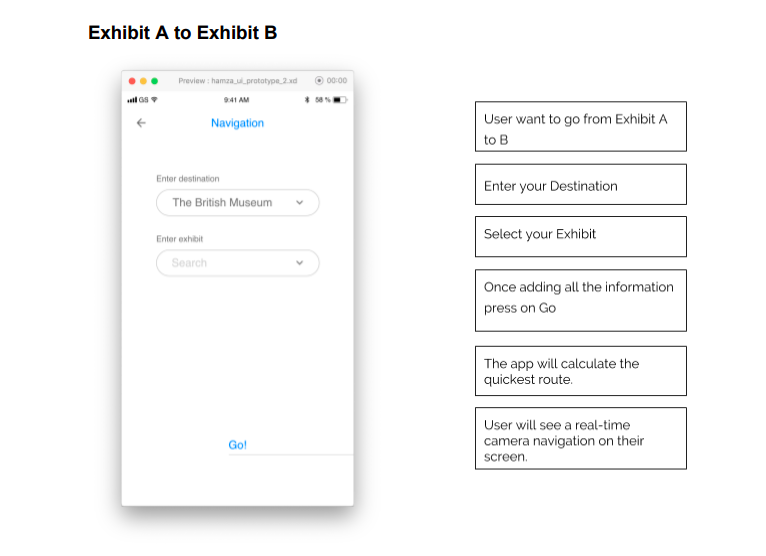
\includegraphics[scale=0.50]{userstory_aTob.png}
    \caption{Going from point A to point B}
    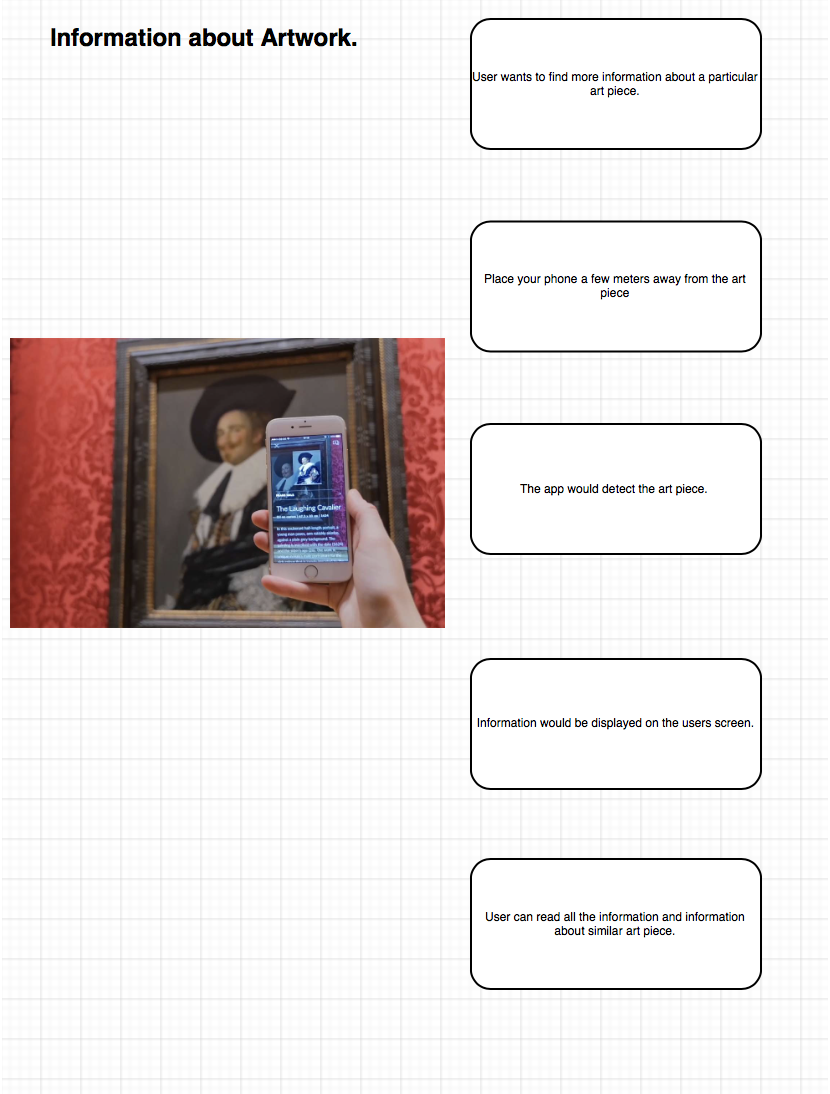
\includegraphics[scale=0.30]{userstory_info.png}
    \caption{Getting information from exhibition}
    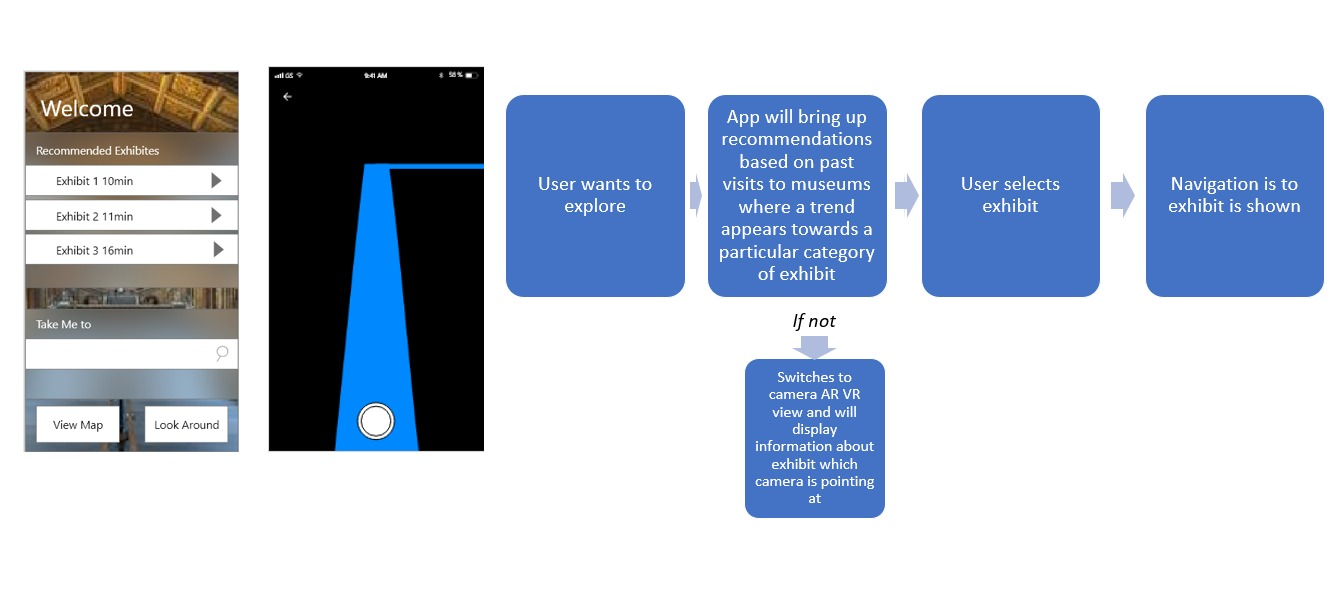
\includegraphics[scale=0.25]{userstory_explore.jpeg}
    \caption{Exploring the museum}
    \label{fig:my_label}
\end{figure}
